\begin{Exercise}[title={Systèmes d'exploitation, gestion des fichiers et des processus}]

Cet exercice traite de l'interaction avec le système d'exploitation, de la gestion des droits, de la surveillance des processus et de l'analyse de réseaux.

\ExePart{Gestion de l'arborescence et des droits d'accès}

On considère l'arborescence de fichiers d'un serveur représentée ci-dessous. Les flèches pointent du répertoire parent vers ses éléments fils.

\begin{center}
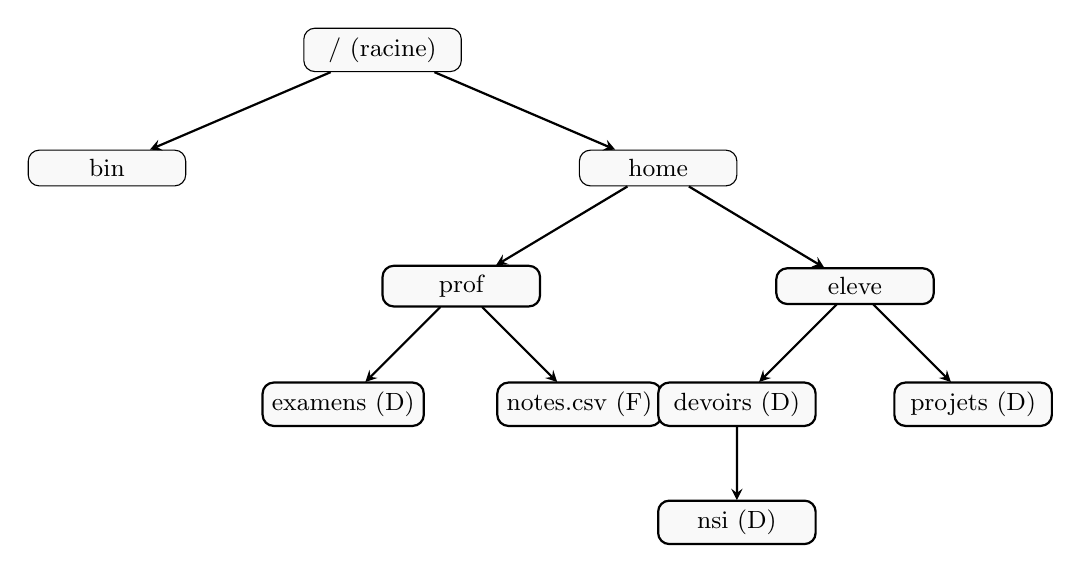
\begin{tikzpicture}[
    every node/.style={draw, rounded corners, fill=gray!5, font=\small, minimum width=2cm},
    edge from parent/.style={draw, -stealth, thick},
    level 1/.style={sibling distance=7cm, level distance=1.5cm},
    level 2/.style={sibling distance=5cm, level distance=1.5cm},
    level 3/.style={sibling distance=3cm, level distance=1.5cm}
]
\node {/ (racine)} 
    child {node {bin}}
    child {node {home}
        child {node {prof}
            child {node {examens (D)}}
            child {node {notes.csv (F)}}
        }
        child {node {eleve}
            child {node {devoirs (D)}
                child {node {nsi (D)}}
            }
            child {node {projets (D)}}
        }
    };
\end{tikzpicture}
\\ \small (D) : Dossier, (F) : Fichier
\end{center}

\Question Un utilisateur est connecté en tant qu'\texttt{eleve}. Son répertoire personnel est \texttt{/home/eleve}. Actuellement, il se trouve dans le dossier \texttt{nsi}.
\begin{enumerate}
    \item Donner le chemin \textbf{absolu} du répertoire \texttt{nsi}.
    \item L'utilisateur souhaite copier le fichier \texttt{notes.csv} (situé chez le \texttt{prof}) vers son propre dossier \texttt{projets}. Écrire la commande en utilisant uniquement des \textbf{chemins relatifs}.
    \item Donner la commande ou la suite de commande permettant de créer (\texttt{touch}) un fichier \texttt{exam1.txt} dans le dossier \texttt{examens}. Pour rappel, vous êtes actuellement dans le dossier \texttt{nsi}.
    \item Vous vous déplacez dans l'arborescence, puis vous tapez la commande suivante. Indiquer ce qu'affiche le terminal.
\begin{lstlisting}[language=bash]
eleve@serveur:~/devoirs/nsi$ ls ../..\end{lstlisting}

    \item L'administrateur exécute la suite de commandes suivante à partir de \texttt{/home/eleve} :
\begin{lstlisting}[language=bash]
$ mkdir archives
$ cd devoirs
$ mv nsi ../archives/
$ ls ../archives\end{lstlisting}
Indiquer ce que la dernière commande affiche à l'écran.
\end{enumerate}

\Question \textbf{Analyse de commandes et droits :}
L'utilisateur tape la commande \texttt{ls -l} dans le répertoire \texttt{/home/prof} et obtient :
\begin{lstlisting}
-rwxrw-r-- 1 prof  enseignants  2048 Mar 24 10:00 notes.csv
\end{lstlisting}
\begin{enumerate}
    \item L'utilisateur \texttt{eleve} (qui n'est pas dans le groupe \texttt{enseignants}) peut-il modifier ce fichier ? Peut-il l'exécuter ? Justifier.
    \item Donner la commande \texttt{chmod} en notation \textbf{octale} permettant de rendre ce fichier lisible et modifiable par tout le monde, mais exécutable par personne.
    \item L'administrateur souhaite transférer la propriété de ce fichier à un autre utilisateur nommé \texttt{directeur}. Il tape la commande suivante :
    \begin{lstlisting}[language=bash]
$ sudo chown directeur notes.csv\end{lstlisting}
    Expliquer le rôle de cette commande et la signification du préfixe \texttt{sudo}.
\end{enumerate}

\ExePart{Processus et Flux de données}

\Question L'administrateur système surveille l'activité et saisit la commande \texttt{ps -ef}. Voici un extrait du résultat :

\begin{center}
\begin{tabular}{|c|c|c|c|c|}
\hline
\textbf{UID} & \textbf{PID} & \textbf{PPID} & \textbf{C} & \textbf{CMD} \\ \hline
root & 1 & 0 & 0 & /sbin/init \\ \hline
root & 500 & 1 & 0 & /usr/sbin/sshd \\ \hline
eleve & 1050 & 500 & 0 & -bash \\ \hline
eleve & 1210 & 1050 & 99 & python3 calcul\_pi.py \\ \hline
eleve & 1215 & 1050 & 0 & ps -ef \\ \hline
\end{tabular}
\end{center}

\begin{enumerate}
    \item Quel est le PID du processus parent de \texttt{python3} ?
    \item \textbf{Dessiner le graphe} de parenté (arbre des processus) pour cet extrait.
    \item Un processus "orphelin" est un processus dont le parent est terminé. Si l'on tue le processus \texttt{bash} (PID 1050), quel processus deviendra le nouveau parent du processus 1210 ?
\end{enumerate}

\Question \textbf{Analyse de commandes complexes :}
On considère la commande suivante : \texttt{ps -ef | grep "python3"}
\begin{enumerate}
    \item Expliquer le rôle du symbole \texttt{|}.
    \item Prédire précisément la sortie de cette commande en utilisant le tableau de la question précédente.
\end{enumerate}

\ExePart{Réseaux et Connectivité}

\Question Pour vérifier la connexion avec un serveur distant, l'utilisateur tape : \texttt{ping -c 3 8.8.8.8}.
Le retour console est le suivant :
\begin{lstlisting}
64 bytes from 8.8.8.8: icmp_seq=1 ttl=115 time=12.4 ms
64 bytes from 8.8.8.8: icmp_seq=2 ttl=115 time=13.1 ms
64 bytes from 8.8.8.8: icmp_seq=3 ttl=115 time=12.8 ms
--- 8.8.8.8 ping statistics ---
3 packets transmitted, 3 received, 0% packet loss, time 2003ms
\end{lstlisting}
\begin{enumerate}
    \item Quel est le rôle de la commande \texttt{ping} ?
    \item Que peut-on conclure sur l'état de la connexion entre l'ordinateur et le serveur 8.8.8.8 ?
\end{enumerate}

\ExePart{Programmation Python et Système}

\Question Dominique souhaite automatiser le nettoyage du serveur. Elle dispose d'une liste de processus représentés par des dictionnaires.

\begin{lstlisting}[language=Python]
processus_actifs = [
    {"pid": 1210, "nom": "python3",
        "cpu": 99.8, "user": "eleve"},
    {"pid": 1340, "nom": "firefox",
        "cpu": 12.5, "user": "eleve"},
    {"pid": 1450, "nom": "bash",
        "cpu": 0.1, "user": "root"}
]
\end{lstlisting}

\begin{enumerate}
    \item Écrire une fonction \texttt{trouver\_critiques(liste\_proc)} qui renvoie une liste contenant uniquement les \textbf{PID} des processus dont la consommation CPU est supérieure à 80 \%.
    \item Dominique veut filtrer les processus par utilisateur. Compléter la fonction suivante :
\end{enumerate}

\begin{lstlisting}[language=Python]
def filtrer_par_user(liste_proc, nom_user):
    resultat = []
    for p in liste_proc:
        if p["user"] == ... :
            resultat.append(...)
    return resultat
\end{lstlisting}


\end{Exercise}